\subsection{Record of the earlier audit}
The following sections retain the earlier donor and switch experiments, released-model diagnostics, native LOCO analysis and clinical query. They document secondary and exploratory results and their original protocol. Claims about the earlier composition-only run refer to that run.

\subsection{Study and analysis scope}
We fixed the original GlaS and HVSMR graph folds and the existing MVTec LOCO partitions before fitting the new readouts. The original gland spacing decomposition was known. The earlier protocol froze the graph contrast, support rules, controls, and useful effect sizes before evaluating the new test scores. The earlier locked graph contrast was edited-state loss AUROC minus absolute probability-change AUROC, with a useful positive gap of at least ten points. The measured contrast reverses that direction. A fixed-model degree intervention was prompted by the test outcome and is exploratory. The visual test and the collateral response distribution use all eligible sources. The common-cell comparison of fault, sham, and deletion was a follow-up to the paired spatial output. The screw-bag extent and the native cardiac term probes are secondary follow-ups.

\paragraph{Paired estimands.}
All graph metrics compare four switch targets with the other pairs within the same graph. The fraction affected and magnitude summaries are computed separately on all targets, added edges, removed edges and untouched pairs. The two-hypothesis AUROC uses half credit for ties. Top-four recall uses fractional allocation to a tied boundary score. Within a source we first average its edits. Within a donor we then average its sources. Donors have equal aggregate weight. The paired bootstrap uses common draw indices across methods and metrics. For image edits, one original photograph and all its variants move together in resampling. Intervals condition on fitted checkpoints and validation cutoffs.

\subsection{Graph construction and matching}
GlaS provides 165 gland instance masks from 16 donors. We use the research-use mirror of the original Warwick-QU challenge files, the supplied donor IDs and $0.620\,\mu$m pixel spacing \cite{glas2017}. Graph adjacency is the undirected union of each gland's two closest annotated boundaries. The sensitivity construction takes the undirected union of its two closest centroids. HVSMR-2.0 uses cropped\_norm v2 in patient RAS axes. Each nonempty structure defines one typed node. Face contact of at least $5\,\mathrm{mm}^2$ defines a link \cite{pace2024}. Part features include log area or volume, elongation, compactness and channel intensity moments.

Of 165 GlaS fields, 140 have at least four nodes, 129 admit a switch, and 78 meet the original 1.35 length criterion. The 60 cardiac graphs all admit a switch and 59 meet the original bound. The saved manifest includes all original switch pairs. For extra edits we enumerate feasible degree-preserving switches on four distinct nodes and choose up to three distinct hash-ordered edits per source. The additional length tier excludes the saved edit. The alternate construction uses the same length criterion. The joint tier tries both assignments of the two additions to the two removals. It minimizes the maximum absolute log ratio across both raw and locally normalized lengths and requires both attributes to agree within a factor of 1.20. An exact role-pair match is prioritized within this bound. In cardiac graphs, each observed role is unique, so each unordered role pair identifies a single candidate. Matching the role-pair multiset exactly would fix the edge set. Cardiac joint switches are distance-matched. \Cref{tab:balance} reports the coverage tradeoff. The CRAG source paper describes an independent gland cohort \cite{graham2019mild}, but the obtainable tiles lacked a verified patch-to-donor key. All new gland edits and constructions therefore reuse GlaS donors.

\begin{table*}[t]
\centering
\caption{\textbf{Coverage, balance, and sensitivity to matching.} D/F/E gives donors, fields or scans, and edits. Raw and local columns give the median and maximum multiplicative imbalance under the \emph{same} correspondence. The original length criterion uses separately sorted raw lengths, so its maximum under the common correspondence can exceed 1.35. Roles counts exact role-pair matches. Gains are against typed centroid distance. Rank minus response compares the GNN's edited-state loss AUROC with its matched absolute probability-change AUROC. Paired intervals are in points.}
\label{tab:balance}
\scriptsize
\setlength{\tabcolsep}{3.5pt}
\begin{tabular}{@{}llrrrrrrr@{}}
\toprule
Cohort & Tier & D/F/E & Raw & Local & Roles & Local gain & Topol. gain & Rank $-$ response \\
\midrule
GlaS & All original & 14/129/129 & 1.18/5.66 & 1.19/6.71 & 258/258 & +11.8 [+8.9, +15.0] & -2.5 [-5.7, +0.8] & -10.5 [-14.4, -6.2] \\
GlaS & Centroid 2-NN & 11/64/120 & 1.21/1.87 & 1.19/1.60 & 240/240 & +15.4 [+11.0, +20.2] & +4.6 [+1.4, +8.1] & -5.1 [-7.1, -2.7] \\
GlaS & Extra length & 11/57/126 & 1.23/1.46 & 1.21/1.54 & 252/252 & +16.1 [+10.4, +22.4] & +4.5 [+0.5, +9.2] & -14.5 [-17.4, -11.7] \\
GlaS & Joint match & 11/36/48 & 1.08/1.20 & 1.08/1.20 & 96/96 & +16.8 [+11.3, +23.0] & +3.2 [-2.6, +9.6] & -17.1 [-22.8, -12.0] \\
GlaS & Original length & 12/78/78 & 1.11/1.58 & 1.10/1.52 & 156/156 & +15.3 [+10.9, +20.1] & +2.1 [-2.4, +7.1] & -16.0 [-19.9, -12.5] \\
\midrule
HVSMR & All original & 60/60/60 & 1.08/1.67 & 1.11/1.83 & 0/120 & +0.4 [-0.2, +1.0] & -5.3 [-6.4, -4.2] & -29.2 [-34.1, -23.8] \\
HVSMR & Extra length & 54/54/146 & 1.19/1.81 & 1.17/1.83 & 0/292 & +0.5 [-0.0, +0.9] & -4.4 [-5.6, -3.4] & -27.9 [-30.7, -24.9] \\
HVSMR & Joint match & 43/43/91 & 1.09/1.19 & 1.08/1.20 & 0/182 & +0.4 [-0.1, +1.0] & -4.2 [-5.4, -3.0] & -29.9 [-34.8, -24.9] \\
HVSMR & Original length & 59/59/59 & 1.08/1.67 & 1.11/1.83 & 0/118 & +0.4 [-0.2, +1.0] & -5.3 [-6.5, -4.1] & -29.5 [-34.5, -24.3] \\
\bottomrule
\end{tabular}

\end{table*}

\paragraph{An exact topology separation.}
Place four same-role parts at consecutive vertices of a unit square and two more at $(0.5,-0.8)$ and $(0.5,1.8)$, using the square from $(0,0)$ to $(1,1)$. Join each horizontal side to its adjacent exterior point to make two triangles. Replace the two horizontal links with the two vertical sides. The result is a six-cycle. Degrees are two in both states. All four switched links have raw length one, and all four square vertices have second-nearest centroid radius one. The multiset of roles, link state, raw distance, and local-normalized distance over all pairs is unchanged. A readout of this multiset must tie. Counting triangles or computing shared-neighbor evidence can distinguish the graphs. This construction isolates topology for this restricted representation.

\begin{table*}[t]
\centering
\caption{\textbf{Earlier graph ranking and response results.} Source and Edited rank targets by the observed-state anomaly score (geometry uses its fixed readout). Response ranks absolute change in conditional probability or change in the geometry readout. The edited intervals are donor paired. GlaS and HVSMR use 78 and 59 source graphs in the original length tier. The pair MLP and frozen GNN controls keep conditional probability fixed.}
\label{tab:previous_graph}
\scriptsize
\setlength{\tabcolsep}{3.5pt}
\begin{tabular}{@{}lrrr@{\hspace{10pt}}rrr@{}}
\toprule
 & \multicolumn{3}{c}{GlaS (78 fields, 12 donors)} & \multicolumn{3}{c}{HVSMR (59 scans, 59 donors)} \\
\cmidrule(lr){2-4}\cmidrule(l){5-7}
Readout & Source & Edited [95\% CI] & Response & Source & Edited [95\% CI] & Response \\
\midrule
Geometry only & 64.0 & 64.0 [57.1, 70.6] & 50.0 & 47.9 & 47.9 [43.4, 52.6] & 50.0 \\
Typed frequency & 61.8 & 61.8 [59.4, 64.2] & 50.0 & 62.4 & 84.5 [81.9, 86.9] & 50.0 \\
Typed distance & 70.1 & 74.9 [70.8, 78.9] & 50.0 & 64.7 & 87.3 [85.1, 89.5] & 50.0 \\
Distance + local spacing & 85.9 & 90.2 [88.4, 91.7] & 50.0 & 65.4 & 87.7 [85.6, 89.7] & 50.0 \\
Handcrafted full context & 80.6 & 85.8 [83.5, 88.0] & 99.3 & 61.2 & 83.5 [81.3, 85.7] & 96.5 \\
\midrule
Pair MLP & 86.7 & 91.5 [89.1, 93.6] & 50.0 & 68.4 & 80.4 [77.9, 83.1] & 50.0 \\
Masked GNN & 77.4 & 82.5 [78.3, 86.5] & 98.5 & 55.5 & 59.4 [56.8, 61.8] & 88.8 \\
GNN, context frozen & 77.4 & 96.2 [95.0, 97.3] & 50.0 & 55.5 & 88.5 [85.6, 91.1] & 50.0 \\
\bottomrule
\end{tabular}

\end{table*}

\subsection{Graph scorers and readout controls}
\paragraph{Fitting.}
Four test folds use the original hash-ordered donor allocation. For each family and fold we sort fitting donors by a second salted hash and take the first quarter, with a minimum of two, for development. The rest fit the two learned link models. Both use donor-balanced BCE, with the per-pair weight inversely proportional to the donor's field count and that field's candidate count. AdamW uses weight decay $0.002$ and batch size 512. Rates $0.002$ and $0.0007$ are compared using the smallest weighted development loss. We train up to 80 epochs with patience 12 and initial seeds 904--907. For GlaS there are nine fit and three development donors per fold. For HVSMR there are 34 and 11. Frozen logistic comparators retain all outer fitting donors and use the original $0.015$ regularization and feature scales.

\paragraph{Frozen references.}
Typed frequency uses add-one smoothing for the binary outcome within each unordered role pair. The typed centroid logit uses role-pair indicators, the log ratio of distance to the graph median distance, and the squared log-distance term. The log ratio is clipped to $[-5,3]$. Context adds the log local-spacing ratio, $\log(1+\mathrm{CN})$, Jaccard overlap, and the logs of one plus the smaller and larger masked degrees. Spacing and topology-only references select the corresponding context features. Feature scales are the fitting standard deviations floored at 0.35. The robust geometry reference uses rolewise medians and $1.4826$ times median absolute deviation floored at 0.15. The three shape descriptors of the part reference have a floor of 0.08 and the remaining intensity descriptors a floor of 0.025. The pooled fit is the fallback for unobserved types. All fits and fold assignments are in the reproduction scripts.

\paragraph{Input and capacity.}
The pair design is the sum of the endpoint one-hot roles, log distance normalized by the median pair distance, and log distance divided by the geometric mean of the two endpoints' local radii. The radii depend only on centroids. Both geometric logs are clipped to $[-5,3]$ in the learned models. The pair-only MLP has hidden widths 60, 60 and 12 with SiLU activations and 5,065 parameters. For the GNN, we copy the adjacency per query, set both directions of the query to zero, and build the two directed neighborhoods from the masked adjacency. For each neighbor the message has its role, both normalized distances to each endpoint, and a bit indicating incidence to the other endpoint. A $13\to32\to24$ SiLU network encodes the messages. For each endpoint we sum messages and divide by $\sqrt{1+\tilde d_i}$. We use the componentwise mean and maximum across endpoints plus the sorted $\log(1+\tilde d_i)$ values. The $60\to48\to24\to1$ head includes the same pair inputs, for 5,369 parameters total. No descriptors, adjacency, or embeddings other than the specified pair inputs enter the MLP. GNN development link AUROC spans 97.4--99.1\% on the original gland graph and 85.1--91.6\% on cardiac. Both models beat the fitting prevalence intercept in all eight original-family folds. The pair MLP meets the 0.80 development AUROC check in all four GlaS and three of four cardiac folds.

\paragraph{Repeatability and held-fixed evidence.}
We checked an observed link and a non-link on every scored source construction. Reversing the bit for the query alone gives identical inputs and an identical conditional probability in 680/680 checks. Repeated scores on the same input had zero drift. Reindexing vertices changes the learned probability by at most $4.77\times10^{-7}$. We use $2\times10^{-6}$ for float32 and $10^{-10}$ for the original float64 score family, consistent with the original similarity and reindexing controls. Numerical ties are distinct from changes of at least $0.10$ development IQR. The IQR is measured on unedited inner development graphs, with a $10^{-3}$ floor. A very small IQR for the observed-state loss can occur when most source non-links are assigned high confidence.

For the GNN, the two paths through observed-state bit $a$ and logit $z$ give direct term $D=-(a'-a)(z+z')/2$ and context term $C=\Delta s-D$. We report $\sum_T|D|/(\sum_T|D|+\sum_T|C|)$ per edit, then aggregate by source and donor. The mean on GlaS is 65.4\% [64.0, 67.2] and on HVSMR 71.1\% [68.1, 74.0]. Some changes cancel between terms. The context-frozen model holds $z$ fixed and reads $s(a',z)$. In GlaS its $|\Delta s|$ ranks all targets first, because its observed query bit is the only changing input. A high response of the loss can therefore differ from a high response of the fitted evidence.

\begin{table*}[t]
\centering
\caption{\textbf{Matched switch sensitivity, direction, and collateral.} $T$ denotes the four targets and $U$ untouched pairs. AUROCs, moved fractions and directional wins are percentages. $W_+$ and $W_-$ summarize additions and removals. The last five columns use development IQR units and report signed mean target shift and absolute shift percentiles. Each percentile is first taken within an edit. The matched scope has 78 fields from 12 gland donors and 59 scans from 59 cardiac donors. Full paired intervals and raw pair scores are retained in the reproducibility data.}
\label{tab:shifts}
\scriptsize
\setlength{\tabcolsep}{2.8pt}
\begin{tabular}{@{}llrrrrrrrrrrrr@{}}
\toprule
Cohort & Readout & Src. & Edited & $\mathrm{AUC}_{|\Delta s|}$ & T moved & U moved & $W_+$ & $W_-$ & Mean $\Delta_T$ & $T_{50}$ & $T_{90}$ & $U_{50}$ & $U_{90}$ \\
\midrule
GlaS & Part appearance & 55.3 & 55.3 & 50.0 & 0.0 & 0.0 & 50.0 & 50.0 & +0 & 0 & 0 & 0 & 0 \\
 & Geometry only & 64.0 & 64.0 & 50.0 & 0.0 & 0.0 & 50.0 & 50.0 & +0 & 0 & 0 & 0 & 0 \\
 & Typed frequency & 61.8 & 61.8 & 100.0 & 100.0 & 0.0 & 100.0 & 0.0 & +0 & 881 & 881 & 0 & 0 \\
 & Typed distance & 70.1 & 74.9 & 100.0 & 100.0 & 0.0 & 30.5 & 79.4 & +0.23 & 2.04 & 2.68 & 0 & 0 \\
 & Distance + local spacing & 85.9 & 90.2 & 100.0 & 100.0 & 0.0 & 41.5 & 76.9 & +0.985 & 4.58 & 6.64 & 0 & 0 \\
 & Distance + topology & 70.6 & 77.0 & 95.7 & 100.0 & 21.6 & 48.3 & 65.2 & +0.423 & 3.43 & 5.61 & 0.00301 & 0.517 \\
 & Handcrafted full context & 80.6 & 85.8 & 98.7 & 100.0 & 21.6 & 51.9 & 70.3 & +1.08 & 5.8 & 9.76 & 0.00116 & 0.309 \\
 & Full context + geometry & 74.6 & 80.1 & 98.7 & 100.0 & 21.6 & 51.9 & 70.3 & +0.369 & 1.85 & 3.11 & 0.0005 & 0.094 \\
 & Pair MLP & 86.7 & 91.5 & 100.0 & 100.0 & 0.0 & 48.9 & 71.2 & +6.79 & 29.5 & 45.7 & 0 & 0 \\
 & Masked GNN & 77.4 & 82.5 & 99.3 & 100.0 & 54.7 & 48.1 & 70.3 & +23.3 & 156 & 307 & 0.0264 & 1.92 \\
 & GNN, context frozen & 77.4 & 96.2 & 100.0 & 100.0 & 0.0 & 73.0 & 82.3 & +290 & 398 & 666 & 0 & 0 \\
\midrule
HVSMR & Part appearance & 53.1 & 53.1 & 50.0 & 0.0 & 0.0 & 50.0 & 50.0 & +0 & 0 & 0 & 0 & 0 \\
 & Geometry only & 47.9 & 47.9 & 50.0 & 0.0 & 0.0 & 50.0 & 50.0 & +0 & 0 & 0 & 0 & 0 \\
 & Typed frequency & 62.4 & 84.5 & 100.0 & 100.0 & 0.0 & 75.4 & 67.8 & +1.78 & 2.71 & 5.07 & 0 & 0 \\
 & Typed distance & 64.7 & 87.3 & 100.0 & 100.0 & 0.0 & 77.1 & 64.4 & +1.45 & 2.05 & 3.84 & 0 & 0 \\
 & Distance + local spacing & 65.4 & 87.7 & 100.0 & 100.0 & 0.0 & 83.9 & 63.6 & +1.49 & 2.14 & 3.94 & 0 & 0 \\
 & Distance + topology & 60.3 & 82.0 & 99.6 & 100.0 & 28.0 & 80.5 & 56.8 & +1.18 & 2.15 & 3.75 & 2.88e-05 & 0.105 \\
 & Handcrafted full context & 61.2 & 83.5 & 99.3 & 100.0 & 28.0 & 81.4 & 57.6 & +1.32 & 2.3 & 4 & 5.78e-05 & 0.0944 \\
 & Full context + geometry & 56.0 & 78.4 & 99.3 & 100.0 & 28.0 & 81.4 & 57.6 & +0.854 & 1.48 & 2.56 & 3.82e-05 & 0.0617 \\
 & Pair MLP & 68.4 & 80.4 & 100.0 & 100.0 & 0.0 & 80.5 & 50.8 & +0.848 & 1.94 & 3.8 & 0 & 0 \\
 & Masked GNN & 55.5 & 59.4 & 85.8 & 100.0 & 77.1 & 76.3 & 38.1 & +0.411 & 2.16 & 4.1 & 0.0874 & 1.33 \\
 & GNN, context frozen & 55.5 & 88.5 & 100.0 & 100.0 & 0.0 & 92.4 & 67.8 & +4.52 & 5.94 & 8.93 & 0 & 0 \\
\bottomrule
\end{tabular}

\end{table*}

\paragraph{Intervening on masked degree.}
Write the original neighborhood vector as the mean message times $\tilde d_i/\sqrt{1+\tilde d_i}$. An empty neighborhood has mean vector zero. The degree-fixed probe uses the edited mean and the source size factor and log degree. The content-fixed probe uses the source mean and the edited factor and log degree. In a degree-preserving switch, a query with unchanged bit has the same masked degree in both states. Consequently the content-fixed intervention changes only the four target queries. These interventions act on fitted network inputs and can create combinations the network did not see in training. \Cref{tab:degree} reports the same protocol on additional edits. Local spacing remains important across constructions, while the learned conditional response has a lower-order cardinality route.

\begin{table*}[t]
\centering
\caption{\textbf{Degree intervention on the fitted GNN.} Response ranks absolute changes in probability. Paired 95\% intervals are shown. Repeated edits reuse the original donors.}
\label{tab:degree}
\scriptsize
\begin{tabular}{@{}lllrrr@{}}
\toprule
Cohort & Tier & GNN comparison & Fields/donors & Response AUROC & Top-four recall \\
\midrule
GlaS & Original length & Full response & 78/12 & 98.5 [97.6, 99.3] & 87.5 [82.4, 92.4] \\
GlaS & Original length & Degree fixed & 78/12 & 85.3 [81.8, 88.9] & 33.7 [25.9, 40.8] \\
GlaS & Original length & Mean messages fixed & 78/12 & 100.0 [100.0, 100.0] & 100.0 [100.0, 100.0] \\
GlaS & Extra length & Full response & 57/11 & 97.6 [95.1, 99.2] & 83.0 [70.0, 91.4] \\
GlaS & Extra length & Degree fixed & 57/11 & 85.4 [80.1, 90.0] & 28.3 [21.3, 34.3] \\
GlaS & Extra length & Mean messages fixed & 57/11 & 100.0 [100.0, 100.0] & 100.0 [100.0, 100.0] \\
GlaS & Joint match & Full response & 36/11 & 98.8 [97.9, 99.6] & 86.6 [80.1, 93.4] \\
GlaS & Joint match & Degree fixed & 36/11 & 87.7 [83.4, 91.9] & 34.7 [23.4, 46.6] \\
GlaS & Joint match & Mean messages fixed & 36/11 & 100.0 [100.0, 100.0] & 100.0 [100.0, 100.0] \\
\midrule
HVSMR & Original length & Full response & 59/59 & 88.8 [85.0, 92.5] & 67.4 [58.5, 76.3] \\
HVSMR & Original length & Degree fixed & 59/59 & 74.3 [70.3, 78.3] & 41.9 [34.7, 49.2] \\
HVSMR & Original length & Mean messages fixed & 59/59 & 100.0 [100.0, 100.0] & 100.0 [100.0, 100.0] \\
HVSMR & Extra length & Full response & 54/54 & 89.9 [87.5, 92.3] & 65.3 [59.5, 70.8] \\
HVSMR & Extra length & Degree fixed & 54/54 & 71.2 [68.8, 73.6] & 34.0 [29.7, 38.1] \\
HVSMR & Extra length & Mean messages fixed & 54/54 & 100.0 [100.0, 100.0] & 100.0 [100.0, 100.0] \\
HVSMR & Joint match & Full response & 43/43 & 90.3 [86.3, 93.8] & 70.4 [61.4, 78.8] \\
HVSMR & Joint match & Degree fixed & 43/43 & 75.3 [71.6, 79.1] & 42.2 [34.7, 50.1] \\
HVSMR & Joint match & Mean messages fixed & 43/43 & 100.0 [100.0, 100.0] & 100.0 [100.0, 100.0] \\
\bottomrule
\end{tabular}

\end{table*}

\paragraph{Earlier motion check.}
The separate V1 perturbation moved one centroid by one median nearest-neighbor spacing while preserving adjacency and all part pixels. Geometry scored 46.8\% target AUROC on 140 GlaS fields from 16 donors and 68.9\% on 60 cardiac scans. Their paired directional wins were 51.2\% and 71.7\%, respectively. This intervention answers a different question from an edge switch and can make some configurations more typical.

\subsection{Photograph interventions and extractor}
The asset mirror retains the official LOCO directory names and RGB photographs. We freeze 372 train/good, 69 validation/good and 138 test/good source identities and fingerprint each image. Training images are split by hash into 302 fitting and 70 inner development images. The visual holdout divides into 63 and 75 test sources by a separate hash. No test score or activation enters candidate selection. The authors' released maps determine the five-column, three-row tray geometry. On the 256-square grid we use $x=(8,57,105,153,201,249)$ and $y=(13,91,166,241)$. Retained pin labels are eight-connected class-2 components of at least 75 pixels. A qualifying source has one per cell. This filter is specific to the compartment experiment.

The RGB cutout is the pin-class component with the neighboring bright pixels from a two-pixel halo, with enclosed holes filled. Selection requires cell clearance and an available local dark background. We fill the original position with the per-channel median of the local dark class-4 ring. Destinations have a one-pixel cell margin, zero overlap with the source cutout or other pins, and at least a two-pixel pin clearance. The oracle component moves entirely onto class 4. The two translations have the same integer squared displacement and equal paste area. The displacement range and intensity thresholds were fixed on validation photographs. In test the moves range from 19.2 to 51.4 pixels. All 138 candidate images meet the edit rules. Sham and fault change exactly the same number of decoded RGB pixels in each pair. Source-pixel repaint is exact. All test masks retain the same class histogram for source, sham and fault. Each move preserves the pin-class component count. All four RGB arms use original camera backgrounds. The held-out scenes contain no generated textures or objects.

The RGB-only extractor is a two-level U-Net with widths 16, 32 and 64, SiLU, group normalization, max pooling and nearest-neighbor upsampling. It predicts six channels. The training label is the released map for each train/good photograph. Weighting is inverse square-root class frequency with floor 0.01. AdamW runs with seed 74817, learning rate $0.001$, decay $0.001$, batch size 12, and at most 30 epochs, selecting the lowest weighted loss on the 70 inner development images. The selected epoch is 30. Development pin IoU is 97.3\% against the released labels and all 70 development images have the correct retained cell counts. On held-out fault maps, pin IoU against the intervened oracle maps is 97.2\%. We keep extraction discrepancies in the test denominator. The extracted arm has its own validation cutoff. Its comparison with the oracle arm includes the effect of re-segmentation and recalibration.

\begin{figure*}[t]
\centering
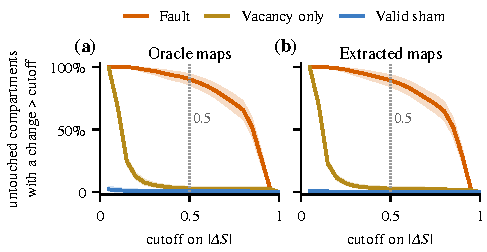
\includegraphics[width=.90\textwidth]{collateral.pdf}
\caption{\textbf{Collateral response across the sigmoid range.} For each fault, deletion, and sham we use the same 13 cells outside the donor and recipient cells. A cell contributes if at least one pixel reaches the specified absolute change. Shading shows original-image-paired 95\% intervals on each fraction. The maximum within a cell measures whether any pixel moves substantially.}
\label{fig:collateral}
\end{figure*}

\paragraph{Reference regions and scene operation.}
The two affected cells are a rule-based coarse spatial reference. The vacant and occupied cells need no pixel-level anomaly outline. For each cell we take the maximum of either the edited output or the absolute change from source. Even the change-based cell rank is 98.4\% on oracle maps while 90.3\% of untouched cells have a large absolute change. The matched deletion, which leaves the same vacancy, keeps changes above $0.5$ to 2.9\% of those same untouched cells. The paired difference is 87.4 points [82.4, 91.9] for oracle maps and 86.6 [81.4, 91.2] after extraction. \Cref{fig:collateral} shows the full threshold curve. These are changes in the spatial output, whereas scene-level maxima and cutoff decisions are a separate measurement.

The image score is the official maximum sigmoid output. The validation IQRs are 0.00974 (oracle) and 0.01060 (extracted). The raw cutoffs are 0.15802 and 0.17097. The rule comparator sums the absolute deviation from one pin per cell and adds retained out-of-grid pins. Its cutoff is zero on both paths. The comparator uses the same labels and the same validation rule. On re-extracted maps it yields zero sham alerts (exact 95\% upper bound 2.6\%), while retaining all 138 fault alerts. \Cref{tab:halves} reports the held-out halves and the paired effect. Figure selection uses the case closest to the median oracle fault-minus-sham score. There were zero missed faults. The second row uses the first hash-ordered alerted sham, whose source also alerts.

\begin{table*}[t]
\centering
\caption{\textbf{Held-out halves for the SALAD photo intervention.} Sham, Fault and Del. count alerts. All fault and deletion recalls are 100\% on the respective support. Bootstrap intervals for tied all-success contrasts are conditional on the sample.}
\label{tab:halves}
\scriptsize
\setlength{\tabcolsep}{3.3pt}
\begin{tabular}{@{}llrrrrrrr@{}}
\toprule
Maps & Split & Sources & Sham & Fault & Del. & Alarm gap (pp) & Paired wins (\%) & Comp. response AUROC \\
\midrule
Oracle & A & 63 & 15 & 63 & 63 & +76.2 [+65.1, +85.7] & 100.0 [100.0, 100.0] & 99.0 [98.4, 99.6] \\
Oracle & B & 75 & 16 & 75 & 75 & +78.7 [+69.3, +88.0] & 100.0 [100.0, 100.0] & 97.9 [96.3, 99.1] \\
Oracle & All & 138 & 31 & 138 & 138 & +77.5 [+70.3, +84.1] & 100.0 [100.0, 100.0] & 98.4 [97.5, 99.1] \\
\midrule
Extracted & A & 63 & 1 & 63 & 63 & +98.4 [+95.2, +100.0] & 100.0 [100.0, 100.0] & 99.2 [98.7, 99.6] \\
Extracted & B & 75 & 6 & 75 & 75 & +92.0 [+85.3, +97.3] & 100.0 [100.0, 100.0] & 98.1 [96.4, 99.1] \\
Extracted & All & 138 & 7 & 138 & 138 & +94.9 [+90.6, +98.6] & 100.0 [100.0, 100.0] & 98.6 [97.6, 99.2] \\
\bottomrule
\end{tabular}

\end{table*}

\subsection{Native LOCO and screw-bag follow-up}
The original SALAD repository checkpoint pair is used for each category. We verified the published download archive, the two checkpoint fingerprints per category, the upstream map decoder, and its unmodified composition forward pass. The maps are indexed labels, mapped to six channels without RGB conversion or interpolation. The expected output is a finite $256\times256$ array in $[0,1]$. In each category the same validation map repeated exactly. The code normalizes the maximum using its normal validation mean and standard deviation. A positive affine transform preserves all rankings and the corresponding validation-order-statistic threshold. The released inputs contain 1,778 fitting, 305 normal validation and 1,568 test entries. The original benchmark paper reports 1,772, 304 and 1,568. We retain the authors' archive splits and retain the authors' published full-system results as context for the original composition-only analysis \cite{fucka2025}.

\begin{table*}[t]
\centering
\caption{\textbf{Native map scores and composition branch alerts.} AUROC in percent. Pos/good counts positives and their eligible negative comparison images. Cutoffs come from normal validation only and stay fixed across scopes. Macro AUROC weights categories equally. Macro alert counts add images. Pushpins has no eligible matched signature.}
\label{tab:locodetail}
\scriptsize
\setlength{\tabcolsep}{4pt}
\begin{tabular}{@{}llrrrrrrrr@{}}
\toprule
Category & Scope & Pos/good & Bag & Grid & Pairs & Extent & SALAD [95\% CI] & Hits & Good alarms \\
\midrule
Breakfast box & Logical & 83/102 & 79.8 & 79.9 & 76.6 & 78.7 & 79.0 [71.6, 85.8] & 53/83 & 15/102 \\
 & Matched & 42/77 & 71.9 & 68.3 & 68.1 & 71.5 & 64.4 [53.4, 75.3] & 17/42 & 14/77 \\
 & Structural & 90/102 & 68.6 & 69.1 & 69.7 & 68.0 & 75.4 [68.2, 82.1] & 48/90 & 15/102 \\
\midrule
Juice bottle & Logical & 142/94 & 84.3 & 85.6 & 85.3 & 83.2 & 88.1 [83.5, 92.1] & 105/142 & 4/94 \\
 & Matched & 99/91 & 82.0 & 84.1 & 85.3 & 82.6 & 82.9 [77.0, 88.4] & 64/99 & 2/91 \\
 & Structural & 94/94 & 74.1 & 70.9 & 68.8 & 66.3 & 85.3 [79.5, 90.6] & 59/94 & 4/94 \\
\midrule
Pushpins & Logical & 91/138 & 77.2 & 76.9 & 73.3 & 67.1 & 99.7 [99.2, 100.0] & 91/91 & 31/138 \\
 & Structural & 81/138 & 56.1 & 59.8 & 53.7 & 50.0 & 76.4 [69.4, 82.9] & 47/81 & 31/138 \\
\midrule
Screw bag & Logical & 137/122 & 76.0 & 76.8 & 63.3 & 61.6 & 90.8 [86.6, 94.4] & 111/137 & 14/122 \\
 & Matched & 79/95 & 75.7 & 75.5 & 58.3 & 56.6 & 90.5 [85.1, 95.4] & 65/79 & 9/95 \\
 & Structural & 82/122 & 71.8 & 76.8 & 67.4 & 66.4 & 85.1 [79.3, 90.2] & 50/82 & 14/122 \\
\midrule
Connectors & Logical & 108/119 & 80.9 & 81.3 & 76.6 & 77.8 & 82.7 [76.8, 88.1] & 74/108 & 9/119 \\
 & Matched & 30/70 & 70.8 & 80.2 & 78.2 & 83.9 & 82.4 [74.6, 89.0] & 21/30 & 6/70 \\
 & Structural & 85/119 & 72.6 & 72.1 & 71.6 & 70.2 & 92.0 [87.8, 95.7] & 69/85 & 9/119 \\
\midrule
Macro & Logical & 561/575 & 79.6 & 80.1 & 75.0 & 73.7 & 88.1 [85.8, 90.2] & 434/561 & 73/575 \\
 & Matched & 250/333 & 75.1 & 77.0 & 72.5 & 73.7 & 80.0 [76.2, 83.8] & 167/250 & 31/333 \\
 & Structural & 432/575 & 68.6 & 69.7 & 66.2 & 64.2 & 82.8 [80.1, 85.4] & 273/432 & 73/575 \\
\bottomrule
\end{tabular}

\end{table*}

The native matched analysis uses the original component rule with an eight-connected minimum of 12 pixels, a catch-all class unseen in fitting, and both test labels plus at least five fitting maps in the signature. Each signature contributes a positive-weighted AUROC within category. The five-nearest-map baselines use blockwise standardized distances and the same training and calibration maps. Counts are per role. The part bag adds log total area and the median and range of log component areas. The grid adds fractional occupancy per role in a $4{\times}4$ grid. The pair block uses the mean coordinate offsets and the 10th, 50th and 90th percentiles of centroid distances by unordered role pair. It uses absolute coordinate offsets within a shared role. Distances are blockwise mean squared standardized differences with training-median imputation. Scale is $1.4826$ times the median absolute deviation, floored at 1.0, 0.25, 0.06 and 0.04 for counts, shapes, grid and pairs, respectively. Average the selected block distances before taking their square roots and averaging the five nearest maps. The extended pair variant uses the same counts and morphology. In the spatial block it averages the original pair distance with distances on absolute centroid position and shape. Position uses the 10th, 50th, and 90th percentiles of each coordinate by role. Extent pools log-transformed bounding spans and square roots of the two coordinate covariance eigenvalues at the same quantiles. The robust spread floors for these added blocks are 0.04 and 0.10. Defined coordinate features and fitted-median imputation follow the original procedure.

\begin{figure*}[t]
\centering
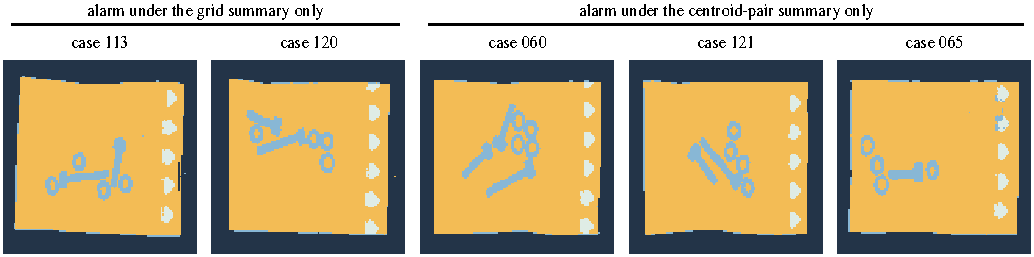
\includegraphics[width=.88\textwidth]{screw_discordant.pdf}
\caption{\textbf{Screw-bag logical cases with discordant grid and centroid-pair alerts.} At the locked thresholds, two of 79 supported faults alert under the grid alone and three under the pair summary alone. The colorized maps show the five cases. Thin fragments around the bag and merged foreground illustrate the difference between predicted counts and physical screw inventory.}
\label{fig:screw}
\end{figure*}

The matched screw-bag cohort has 79 faults and 95 good maps. Pairs trail the grid by 17.1 points [$-24.9$, $-9.0$] from unrounded scores (17.2 from rounded table entries). The other three categories average about $-0.3$ points. Adding placement and extent gives 56.6\% versus 58.3\% for the original pair block and 75.5\% for the grid. The paired difference relative to the original pair block is $-1.7$ points [$-9.9$, $+6.3$]. In \cref{fig:screw}, the predicted metal role includes narrow boundary fragments and can merge physical parts. For example, the largest projected long-axis extent in case 121 belongs to a 143-pixel fragment along the image-side edge. Per-role pooled extent therefore cannot identify the actual length of each screw. This probe supports a limit of the tested summaries on the supplied maps. In the native full comparison the grid's logical recall is 51.5\% macro with 11.1\% good alerts, versus 53.3\% and 10.3\% for the bag. Matched SALAD minus grid is $+3.0$ points [$-2.1$, $+8.2$] across the four supported categories and $+15.1$ [5.9, 24.5] in screw bag.

\subsection{One native SVC--PA query}
The code comparison keeps five negative fit patients, 20 negative calibration patients, and test patients with 24 Glenn codes and ten without. Mask face contact has 100\% test AUROC, detects 24/24 positives [85.8, 100], and alerts on 1/10 code-negative scans [0.25, 44.5]. The $31.47\,\mathrm{mm}^2$ calibration threshold is below the largest negative ($48.45$) and smallest positive ($58.17$). Axial-mask profiles detect 21/24 with zero negative alerts. Full contextual loss has 19.6\% AUROC and detects 0/24 at its cutoff. Its masked link probability is higher on the Glenn-coded test scans (median 0.712 versus 0.441). Refitting without the degree terms raises AUROC to 44.2\%. Removing the shared-neighbor terms gives 18.3\%. Distance alone gives 75.4\%. Removing one incident link at a time while holding the SVC--PA bit fixed yields mean absolute within-patient probability shifts of 0.093 on the 21 Glenn-coded patients with at least one such link and 0.144 on ten code-negative patients. These are exploratory sensitivity checks on five fit patients and a single query. They do not resolve the causal effects of surgery. Five target-negative SVC variants occur in the release, with two in fit and three in calibration. The test has zero. Independent adjudication of native relations and benign variants is needed to extend the scope beyond this code.

